\documentclass[10pt]{article}
\usepackage{amsmath}
\usepackage{fancyhdr}
\usepackage{amsthm}
\usepackage{scalerel} %调整积分符号大小
\usepackage{tikz}
\usepackage{bm}
\usepackage{lipsum}
\usepackage{tcolorbox}
\usepackage{mathrsfs}
\usepackage{xeCJK}
\usepackage{graphicx}
\setCJKmainfont{PingFangSC-Light}
\newcommand*\circled[1]{\tikz[baseline=(char.base)]{
            \node[shape=circle,draw,inner sep=2pt] (char) {#1};}}
\newcommand{\hilight}[1]{\colorbox{yellow}{#1}}
\usepackage{ amssymb }
\usepackage[utf8]{inputenc}
\usepackage[english]{babel}
\usepackage{color}
\usepackage[left=1in,top=1in,right=1in,foot=1in]{geometry}
\usepackage{graphicx}
\setCJKmainfont{Kai}
\newenvironment{changemargin}[2]{%
  \begin{list}{}{%
    \setlength{\topsep}{0pt}%
    \setlength{\leftmargin}{#1}%
    \setlength{\rightmargin}{#2}%
    \setlength{\listparindent}{\parindent}%
    \setlength{\itemindent}{\parindent}%
    \setlength{\parsep}{\parskip}%
  }%
  \item[]}{\end{list}}
\renewcommand{\arraystretch}{1.1}
\setlength\parindent{0in}
\pagestyle{fancy}

\fancyhf{}
\lhead{MATH\,316\,\,\, PDE 偏微分方程}
\rhead{\scriptsize{\copyright \,Shihao Tong All Right Resvered}}
\rfoot{Page \thepage}
\renewcommand{\headrulewidth}{0.5pt}



\begin{document}

\theoremstyle{definition}
\newtheorem{definition}{Definition}

\theoremstyle{lemma}
\newtheorem{lemma}{Lemma}

\theoremstyle{theorem}
\newtheorem{theorem}{Theorem}



%\begin{flushright}
%  % EDIT THIS NEXT LINE: Replace ``Name'' with your own name
%%   \large{\textbf{Shihao Tong (Owen)}}
%% \\
%  % EDIT THIS NEXT LINE: Replace ``12345678'' with your own student number
%%   \large{\textbf{38191201}}
%\end{flushright}

% Edit this line for title
%\large{\textbf{Stat 305 Statistical Inference}}

\def\stretchint#1{\vcenter{\hbox{\stretchto[400]{\displaystyle\int}{#1}}}}
\def\scaleint#1{\vcenter{\hbox{\scaleto[4ex]{\displaystyle\int}{#1}}}}
%
%\normalsize


%\begin{tabular*}{6.5in}{c}
%\hline
%\end{tabular*}
%
%\bigskip

\begin{changemargin}{-0.125in}{0in}



\begin{enumerate}
	
	\item \textbf{Cauchy-Euler/ Equid-imensional Equation}
	
	\medskip
	
	This is a case of second order non-constant coefficient partial differential equation. The from of PDE is 
	\[
	\mathcal{L} \,y = x^2\cdot y'' + \alpha x \cdot y' + \beta y = 0
	\] 
	where $\alpha, \beta \,\in \mathcal{R}$. The guessed solution is 
	\[
	y(x) = x^r,\,\,\,\, r\in \mathcal{R}
	\]
	
	By substitution we have 
	\[
	\mathcal{L}\,y(x) = r(r-1)x^r + \alpha r\cdot x^r + \beta x^r = [r^2 + (\alpha -1) r + \beta] x^r = 0
	\]
	Since $x^r$ can not be zero (we don not want a trivial solution), so now we get the \textit{characteristic equation}
	
	\begin{tcolorbox}[notitle,boxrule=0pt,colback=blue!20,colframe=blue!20]
       \[
       r^2 + (\alpha -1)r + \beta
       \]
       \end{tcolorbox}
       
       
       A more general representation can be this: The Equation is $\mathcal{L}\,y = \lambda x^2\cdot y'' + \alpha x\cdot y' + \beta y = 0$ which is more general than previous one. Then with the same approach (assume the solution is $y = x^r$) we find the characteristic equation is 
       \begin{tcolorbox}[notitle,boxrule=0pt,colback=blue!20,colframe=blue!20]
       \[
       \lambda r^2 + (\alpha - \lambda)r + \beta
       \]
       \end{tcolorbox}
       where $\lambda$ is simply 1 in the simplest form.
       \medskip
       
     Then we apply the same logic as in ODE analysis, the general solution should be the linear conbination of all possible solution. Also, because the char. eq is quadratic, we can discuss it under three cases depending on discriminant $\Delta$, which is 
     \[
     \Delta = \frac{- (\alpha -1) \pm \sqrt{(\alpha - 1)^2 - 4\beta}}{2}
     \]
     
     \begin{itemize}
     	\item $\Delta > 0$: Two distinct real roots, then 
        \begin{tcolorbox}[notitle,boxrule=0pt,colback=orange!20,colframe=blue!20]
     	\[
     	y_g(x) = C_1 x^{r_1} + C_2 x^{r_2}
     	\]
     	\end{tcolorbox}
        \item $\Delta < 0$: Two complex roots. Then similar to the case in ODE, we want to apply the Euler's Equation to represent the solution in terms of trig. functions. So 
        \[
        y_g(x) = C_1 x^{r_1} + C_2 x^{r_2} = C_1 x^{\lambda + \mu i} + C_2 x^{\lambda - \mu i}
        \]
        where $\lambda = -(\alpha -1)/2$ and $\mu = \sqrt{4\beta - (\alpha -1)^2}$. Then 
        \[
         = C_1 \cdot e^{(\lambda + \mu i)\ln x} + C_2 \cdot e^{(\lambda - \mu i)\ln x} 
        \]
        \[
         = e^{\lambda \ln x }\big(C_1 e^{\mu\ln x \cdot i} + C_2 e^{-\mu\ln x \cdot i}\big)
        \]
        applying the Euler's Equation we have 
        \[
         = x^\lambda \big[(C_1 + C_2)\cos(\mu \ln x) + i \cdot (C_1 - C_2)\sin (\mu \ln x)\big]
        \]
        we focus only on the real part (by thinking of $C_1 + C_2$ and $C_1 - C_2$ can be complex and multiply by $i$ can produce a real coefficient). So the general solution is 
        \begin{tcolorbox}[notitle,boxrule=0pt,colback=orange!20,colframe=blue!20]
        \[
        y_g(x) = x^\lambda [A_1 \cos(\mu \ln x) + A_2 \sin (\mu \ln x)]
        \]
        \end{tcolorbox}
        Notice is $x < 0$, then replace all $x$ by $|x|$ (because of $\ln$).
        
        \smallskip
        
        \item $\Delta = 0$: Two equal real roots. So we want to find a another solution which is linear independent to $y_1 (x) = x^{r_1}$. The way we find the second solution is based on the property of linear operator which is 
        \[
        \mathcal{L}\,\frac{\partial}{\partial r} (y) =\frac{\partial}{\partial r} \,\mathcal{L} (y)
        \]
        So the logic is: we start with the RHS $\mathcal{L}$ by plugging into $y(x) = x^r$ ($r$ is general here), then take the derivative of it and set the LHS equals to it. The process is 
        \[
        \mathcal{L}\,y(x,r) = \mathcal{L} x^r = [r^2 + (\alpha -1)r + \beta]x^r  
        \]
        \[
        = 
        \big[(r + \frac{\alpha -1}{2})^2 - \frac{(\alpha -1)^2 - 4 \beta}{4}\big]x^r
        \]
        where we construct such a square form where the second part in the bracket equals 0 since $\Delta = 0$. Then 
        \[
        = (r - r_1)^2x^r = (r - r_1)^2e^{r\ln x}
        \]
        Then we have 
        \[
        \frac{\partial}{\partial r} \mathcal{L}(y(x,r)) \big| _{r = r_1}= 2(r - r_1)x^r + (r - r_1)^2 \ln x e^{r \ln x}  = 0
        \]
        then
        \[
        \frac{\partial}{\partial r} y(r,x) \big| _{r = r_1} = x^{r_1} \ln x \longrightarrow  \mathcal{L} ( x^{r_1} \ln x ) =0
        \]
        which means the partial derivative regards to $r$ of $y(r,x)$ is also a solution to the PDE. Thus the general solution is 
        \begin{tcolorbox}[notitle,boxrule=0pt,colback=orange!20,colframe=blue!20]
        \[
        y_g(x) = C_1 x^{r_1} + C_2 x^{r_1} \ln x
        \]
        \end{tcolorbox}
      \end{itemize}
      
      The way to check two solution is linearly independent or not is using the \textit{Wronskian} \textcolor{red}{made up later}.
      
      \medskip
      
      \medskip
      
      \item \textbf{Series solution of ODES}
      
      \smallskip
      
      Similar to Taylor expansion, we can use a power series to approximate the solution of the Variable coefficient linear ODE's. The approximation is using 
      \[
      f(x) = \sum_{n=0}^\infty\,a_n (x - x_0)^n
      \] 
      where $a_n's \in \mathcal{R}$. Since the sum is infinite until $n \rightarrow \infty$, so it is exactly equals, or we can use some finite terms to do the approximation. $x_0$ is the $center$ we chose to do the expansion. 
      
      \medskip
      
      Recall the \textit{Ratio test}, which is used to test whether the series is absolutely convergent or not 
      \[
      \lim_{n\rightarrow\infty}\,\, \bigg| \frac{a_{n+1} (x - x_0)^{n+1}}{a_n (x-x_0)^n} \bigg| = \big|x-x_0\big| \lim_{n \rightarrow \infty}\bigg|\frac{a_{n+1}}{a_n}\bigg|
      \]
	  if this ratio is less than one, then the series convergent absolutely (convergent but not absolutely if $a_{n+1}/a_n<1$, 无绝对值号). If further, we know the series absolutely converges for $|x - x_0|< \rho$, then we say the \textit{radius of convergence is $\rho$}.
	  
	  \medskip
	  
	  \begin{enumerate}
	  
	  \item \textbf{Taylor series}
	  
	  \smallskip
	  
	  Now we assume the function $f(x)$ that we want to approximate is continuous and has all higher order derivatives fof $|x - x_0| < \rho$ (within the convergence radius), then by using a power series approximation we can write 
	  \[
	  f'(x) = \sum_{n = 1}^\infty a_n(x - x_0)^{n-1}
	  \]
	  \[
	  f''(x) = \sum_{n = 2}^\infty n(n-1)a_n(x - x_0)^{n-2}
	  \]
	  \[
	  f^{(3)}(x) = \sum_{n=3}^\infty n(n-1)(n-2) a_n(x - x_0)^{n-3}
	  \]
	  then we find 
	  \[
	  f'(x_0) = a_1,\,\,f''(x_0) = 2\,a_2,\,\,f^{(3)}(x_0) = 3!\,a_3
	  \]
	  and in general, we have 
	  
	  \begin{tcolorbox}[notitle,boxrule=0pt,colback=blue!20,colframe=blue!20]
	  \[
	  f^{(n)}(x_0) = n! \cdot a_n \implies a_n = \frac{f^{(n)}(x_0)}{n!}
	  \]
	  \end{tcolorbox}
	  finally we have 
	  \[
	  f(x) = \sum_{n = 0}^\infty \,\frac{f^{(n)}(x_0)}{n!} \cdot (x - x_0)^n
	  \]
	  the Taylor series of $f(x)$ at the point $x_0$. We say $f(x)$ is \textit{analytic} at $x = x_0$ if the radius of convergence of the Taylor series of $f(x)$ is $\rho > 0$.
	  
	  \smallskip
	  
	   \begin{tcolorbox}[notitle,boxrule=0pt,colback=orange!20,colframe=blue!20]
	   Notice: We want to expand/approximate the function at a point which is convergent, since if it is not convergent, the sum of series will be infinite, then we can not use it to approximate the function.
	   \end{tcolorbox}
	   
	   \smallskip
	   
	   \item \textbf{Series Solution of ODES}
	   
	   \smallskip
	   
	   Instead of Taylor expansion, we usually use the \textit{Maclaurin expansion}, which is the Taylor expansion at $x_0 = 0$. It is useful since in many cases, the radius of convergence is $\infty$, which means the series is convergent everywhere and using $x _0 = 0$ is usually easy to compute. 
	   
	   \medskip
	   
	   The basic idea here is this. Given a ODE, we first guess a solution in form of power series (e.g $f(x) =a_nx^n$), then using the ODE to find all the coefficient of the power series which is equivalent to some solution. 
	   
	   \bigskip
	   
	   \underline{\textbf{{EXAMPLE1.}}} \,\,\, Solve the ODE $y' = 2y$ by power series. 
	   
	   \medskip
	   
	   \underline{\textbf{SOLUTION.}} \,\,\, Assume the solution $y = \sum_{n=0}^\infty\,a_n x^n$. Then 
	   \[
	   y'(x) = \sum^\infty_{n = 1}\,\, n \cdot a_n x^{n-1}
	   \]
	   plug in to he ODE we have 
	   \[
	   \sum^\infty_{n = 1}\,\, n \cdot a_n x^{n-1} - 2 \sum_{n=0}^\infty\,a_n x^n = 0
	   \]
	   Notice the index are different. One starts from 1 and the other from 0. No matter in with summation, all $a_i$'s explicitly refer to the same coefficient, since they are all generated from the basic solution we assumed above. So we shift the index. This make both sum start form 0. Let $m = n - 1$, then
	   \[
	   \sum^\infty_{n = 1}\,\, n \cdot a_n x^{n-1} - 2 \sum_{n=0}^\infty\,a_n x^n = \sum^\infty_{m = 0}\,\,(m+1) \cdot a_{m+1} x^{m} - 2 \sum_{m=0}^\infty\,a_m x^m
	   \]
	   \[
	   \sum_{m=0}^\infty\, x^m[(m+1)a_{m+1} - 2 \cdot a_m] = 0
	   \]
	   appealing to the property of \textit{linearly independent}, each of all the coefficient must be zero to make the sum be zero (since all $x_i$'s are linearly independent). So 
	   \[
	   a_{m + 1} = \frac{2}{m+1} a_m \implies a_n = \frac{2^n}{n!}a_0
	   \]
	   this is a \textit{recurrence relation} (may be prove more rigorous by induction). Plug these coefficient into our assumed solution we have 
	   \[
	   y(x) = \sum^\infty_{n = 0} \,\,a_n x^n = \sum^\infty_{n = 0} \frac{2^n}{n!} a_0 \cdot x^n = \sum^\infty_{n = 0} \frac{(2x)^n}{n!} a_0 = a_0 e^{2x}
	   \] 
	   Then, in order to show this is a valid solution, we have to do the ratio test to check the radius of convergence, which is 
	   \[
	   \lim_{n \rightarrow \infty} \, \big|  \frac{a_{n+1}x^{n+1}}{a_n x^n}  \big| = \lim_{n \rightarrow \infty}\,\big|\frac{(2x)^{n+1} n! a_0}{(2x)^n (n+1)! a_0}  \big| = \lim_{n \rightarrow \infty} \big|\frac{2x}{n+1}\big| = 0 < 1
	   \] 
	   thus converges everywhere (center at $x_0 = 0$ with radius of convergence = $\infty$).t
	   \medskip
	   
	   \begin{tcolorbox}[notitle,boxrule=0pt,colback=orange!20,colframe=blue!20]
	   Notice: A trick here sometimes can be this: the power of $x$ in each summation may not match even after shifting of index. In order to find a recursion relation in the similar way as previous, one way to do is take the first term (which is always constant) out of the summation such that the remaining terms will match. 
	   \end{tcolorbox}
	   
	  \end{enumerate}
	  
	  \item \textbf{The Airy Equation} 
	  
	  \[
	  \mathcal {L} y = y'' - xy = 0
	  \]
	  \underline{Solution:} \,\,The solution can be find via series solution. We assume the solution exists and in a form of power series which is $y(x) = \sum^\infty_{n =0}$. Then as regular compute the first \& second derivative and plug into the ODE, we get 
	  \[
	  \mathcal{L}\,y = \sum^{\infty}_{n = 0}a_n\cdot n(n - 1)x^{n-2} - \sum^{\infty}_{n = 0}a_nx^{n+1}
	  \]
	  We have to shift the index to match the power (Notice: we usually shift the one with lower power to the higher one). $x^{n+1}$ is our target. Thus let $m + 1 = n-2$, the summation becomes 
	  \[
	  = \sum_{m = -1}^{\infty} \,a_{m+3} (m+3)(m+2)x^{m+1} - \sum^\infty_{n = 0}a_nx^{n+1}
	  \]
	  Both series should start from the same index, so take out the first term inside the first summation, which leads to 
	  \[
	   = 2\cdot a_2 x^0 + \sum^\infty_{m = 0} \, [a_{m+3} (m+3)(m+2) -  a_m]x^m
	  \]
	  Since all $x^i$'s are linearly independent (including $x^0$), all coefficient have to be zero, which is 
	  \[
	  a_2 = 0,\,\,\,\& \,\,\,a_{m+3} (m+3)(m+2) -  a_m = 0 \implies a_{m+3} = \frac{a_m}{(m+3)(m+2)}
	  \]
	  the recursion soliton does not have a very particular pattern however we can finally find the coefficients are all able to be expressed in terms of $a_1$ and $a_0$. The general solution looks like 
	  \[
	  y(x) = a_0(1 + \frac{x^3}{6} + \frac{x^6}{180} + ...) + a_1(x + \frac{x^4}{12} + \frac{x^7}{504} + ...)
	  \]
	  finally check the radius of converges we get 
	  \[
	  \lim_{n \rightarrow \infty} \big| \frac{a_{m+3}x^{m+3}}{a_m x^m}\big|
	  \]
	  \textcolor{red}{question: with m+3/m not m+1/m? }\textcolor{blue}{Answer: want the ratio between two consecutive term in the summation of serie}
	 
	  
	  \medskip
	  
	  
      \hilight{\textbf{Example:(C-E Equation)}} \,\,\.Solve $(x - 1)y'' + y' = 0$. 
	  
	  \medskip
	  
	   This is exactly a C-E Equation with $\beta = 0$ if we multiply $(x -1)$ on both side (the ODE becomes equal dimensional). Since the first term is $(x-1)^2\cdot y''$, so we can guess the solution is in form of 
	   \[
	   y_h(x) = (x - 1)^r
	   \]
	   then consequently we have 
	   \[
	   y'_h(x) = r(x - 1)^{r-1},\,\,\, y''_h(x) = r(r-1)x^{r-2}
	   \]
	   substitute into the ODE we have 
	   \[
	   [r(r-1) + r] (x-1)^r = 0 \implies r(r-1) + r = 0 \implies r_{1,2} = 0
	   \]
	   by our discussion for C-E equation, the general solution is 
	   \[
	   y_h(x) = C_1 + C_2 \ln |x-1|
	   \]
	   Now use the power series to find the solution (\hilight{a nice example for shifting index}). As what we do regularly, guess solution as a power series $y(x) = \sum^\infty_{n=0} a_nx^n$. Then take derivatives and plug in we get 
	   \[
	   -\sum_{n=2}^\infty \,a_n n (n-1) x^{n-2} + \sum_{n=2}^\infty \,a_n n (n-1) x^{n-1}   + \sum_{n=1}^\infty a_n n x^{n-1}
	   	   \]
	   	   We first shift the index to match the power. As we suggested to shift the lower to higher ($n-2$ to $n-1$). Let $m-2 = n-1$, then 
	   	   \[
	   	   = -\sum_{m=1}^\infty \,a_{m+1} (m+1) m x^{m-1} + \sum_{m=2}^\infty \,a_m m (m-1) x^{m-1}   + \sum_{m=1}^\infty a_m m x^{m-1}
	   	   \]
	   	   Then each of the summation should start from the same index. So take out the first term from the first and third summation and fortunately they are constant. Then we get 
	   	   \[
	   	   (a_1 - 2a_2) + \sum_{m=2}^\infty \, [a_{m}m^2 - a_{m+1}(m+1)m]
	   	   \] 
	   	   since linearly independent, we have 
	   	   \[
	   	   a_1 = 2a_2,\,\,\&\,\,a_{m+1} = a_m \cdot \frac{m}{m+1} 
	   	   \]
	   	   by induction (if formally), the general solution for coefficient is 
	   	   \[
	   	   a_n = \frac{a_1}{n}
	   	   \]
	   	   notice, the ODE after plugging in the derivatives \hilight{does not include information about $a_0$, so it means $a_0$} \hilight{can be arbitrary.} So the solution become 
	   	   \[
	   	   y(x) = a_0 +  a_1\sum^\infty_{n =1} \,\frac{x^n}{n} =a_0 - a_1 \ln |1-x| 
	   	   \]
	   	   \textcolor{red}{why last equality}. Check the radius of convergence we find 
	   	   \[
	   	   \lim_{n\rightarrow \infty}\,\bigg| \frac{x^{n+1}n}{x^n (n+1)} \bigg| = | x | < 1 \,\,\implies\,\, -1<x<1
	   	   \]
	   	   so the radius of convergence is 1 and the series converges on $x \in (-1,1)$ (expanded around 0). 
	   	   
	   	   \medskip
	   	   
	   	   上述例子中有一个问题,即在用ratio test时没有检验两个收敛半径的端点值1和-1。通过带入发现$x=1$时是调和级数,发散;而$x =-1$时收敛。因此$x=-1$也合理。
	   	   
	   	   \medskip
	   	   
	   	   另外我们尝试在$x+0 = 1$处展开以寻找ODE的解。发发现得到$a_n = 0$。所以在1处展开不能得到ODE的解。我们称$x_0 = 1$为\textit{singular point},称任意$x_0 \neq -1$为\textit{an ordinary point}。 注意 
	   	   \begin{itemize}
	   	   	\item A power series solution is possible for all ordinary points, but not for all singular points.
	   	   	\item The radius of convergence of the poser series solution is at least as large las the distance from $x_0$ to the nearest singular point.
	   	   \end{itemize}
	   	   
	   	   singular point是指在ODE中,能使$P(x) = 0$ 的点,ordinary point是指在周围展开可以得到合理的解且不使$P(x)=0$的点。但是有时候在\textit{singular point}处也能得到合理的解。
	   	   
	   	   \medskip
	   	   
	   	   \item \textbf{Series solutions of 2nd order Variable-coefficient linear ODEs}
	   	   
	   	   \medskip
	   	   
	   	   We are going to solve the 2nd ODE in form like 
	   	   \[
	   	   \tilde{P}(x) + Q(x)y' + R(x)y = 0
	   	   \]
	   	   and transform it into 
	   	   \[
	   	   y'' + p(x)y' + q(x) = 0
	   	   \]
	   	   where where divide each coefficient by $P(x)$. Then 
	   	   \begin{itemize}
	   	   	\item If $p(x)$ and $q(x)$ are both analytical at $x_0$, then $x_0$ is an \textit{ordinary} point for the solution of ODE (i.e both function can be expanded at $x_0$ and has all valid higher order derivatives). This means the solution of the ODE is in form of
	   	   	\[
	   	   	y(x)= \sum_n a_n(x-x_0)^n = a_0y_1(x) + a_1y(x)
	   	   	\] 
	   	   	 which is the linear combination of two solution ($y_1$与$y_2$线性无关). 
	   	   	
	   	   	\medskip
	   	   	
	   	   	\item If $p(x)$ and $q(x)$ are not analytical (i.e $\tilde{P}(x_0) = 0$), then $x_0$ is an \textit{singular} point, which means no valid series solution at $x_0$.
	   	   	
	   	   	\smallskip
	   	   	
	   	   	Also appealing to previous discussion, if $x_0$ is ordinary, the radius of convergence is at least as large as the distance form $x_0$ to the nearest singular point.
	   	   \end{itemize}
	   	   
	   	   \medskip
	   	   
	   	   Singular point can be classified into tow categories: 
	   	   \textit{regular} singular point \& \textit{irregular} singular point. For regular singular point, the solution can be found by using Forbenius series, while the irregular one is beyond this course. 
	   	   
	   	   \begin{tcolorbox}[notitle,boxrule=0pt,colback=orange!20,colframe=blue!20] 
	   	   \begin{definition} (Regular Singular Points) Assume the ODE is same as what we defined at the very beginning. Then $x_0$ is regular singular point if
	   	   \[
	   	   \lim_{x\rightarrow x_0}\,(x-x_0)\frac{Q(x)}{\tilde{P}(x)} \neq \infty,\,\,\&\,\,\lim_{x\rightarrow x_0}\,(x-x_0)^2\frac{R(x)}{\tilde{P}(x)}\neq \infty
	   	   \] 
	   	   $x_0$ is irregular if either or both of the limit is infinite. 
	   	   
	   	   \end{definition}
	        \end{tcolorbox}
	        
	        We transform the equation at the beginning to be \[
	            (x - x_0)^2 y'' + \frac{Q(x)}{\tilde{P}(x)}(x - x_0)^2 + \frac{R(x)}{\tilde{P}(x)}(x-x_0)^2 =0
	            \]
	            \[
	            \implies (x - x_0)^2 y'' + p(x)(x - x_0)y' + q(x)y =0
	            \]
	            where $p(x)$ and $q(x)$ are the part we check to determine the singularity. 
	            
	            
	            \bigskip
	            
	            \item \textbf{Frobenius series solution near regular singular point}
	            
	            \medskip
	            
	            \begin{definition}
	            	Let $x_0$ is a regular singular point of the ODE $ \tilde{P}(x) + Q(x)y' + R(x)y = 0$, then the Frobenius series solution is in form of 
	            	\[
	            	y(x) = (x-x_0)^r\sum_{n=0}^\infty \,a_n (x-x_0)^n
	            	\]
	            \end{definition}
	            In order to find the solution we need to \circled{1} Find the value for $r$ \circled{2} Find the recurrence relation of $n$ \circled{3} Find the radius of convergence of $)^r\sum_{n=0}^\infty \,a_n (x-x_0)^{n + r}$
	            
	            
	            \bigskip
	            
	            \item \textbf{Bessel's Equation: PDE application}
	            
	            \medskip
	            
	            The Bessel's equation is in form 
	            
	            \[
	            \mathcal{L} y = x^2y'' + xy' + (x^2 - v^2)y = 0
	            \]
	            where $v$ is the order of the Bessel function which is not an integer. It is easy to check $x=0$ is a regular singular point. We have tow methods to deal with such case: one by approximation and one by Frobenius series. \textcolor{blue}{Approximation make up later}So use $y = \sum^\infty_{n=0}a_n x^{n+r}$ (Frobenius seies). After plugging in the derivatives we get 4 cases: \circled{1} $r = v, v = 1/2$, \circled{2} $r = v, v = -1/2$, \circled{3} $r = -v, v = 1/2$, \circled{4} $r = v, v = 1/2$. For case two and three, $a_1$ is arbitrary. 	            
	            \medskip
	            
	            \begin{itemize}
	            	
	             \item \textbf{Case1: $r = \pm v$ and $v \neq \pm 1/2$}\,\,\\
	             
	             
	            For $r = v$ we can find the recurrence relation and then the solution 
	            \[
	            y_1(x) = a_0 x^v \,\sum^\infty_{m=0}\,\frac{(-1)^m x^{2m}}{m!\, 2^{2m}(1+v)(2+v)...(m+v)}\,\,\,\,\,\&\,\,\,\,\lim_{x_0 \rightarrow 0} y_1(x) \rightarrow 0
	            \]
	            For $r = -v$ we can find the recurrence relation is 
	            \[
	            y_2(x) =a_0 x^{-v} \,\sum^\infty_{m=0} \frac{(-1)^m x^{2m}}{m!\,2^{2m}(1-v)(2-v)...(m-v)}\,\,\,\,\,\&\,\,\,\,\lim_{x_0 \rightarrow 0} y_2(x) \rightarrow \infty
	            \]
	            
	            \item \textbf{Case2: $v = 0$} The indicial equation has double root: $r_1 = r_2 = 0$ (indicial equation is the corresponding Cauch Euler equation of the ODE, the cases of root of the indicial equation determine the form of the general solution of the ODE). The solution in this case is 
	            \[
	            y_1(x) = x^0\,\sum^\infty_{m=0}\frac{(-1)^m a_0x^{2m}}{2^{2m}(m!)^2} = J_0(x)
	            \]
	            $J_0(x)$ is known as the \textit{Bessel function of the first kind of order zero}. The solution can also be found by plugging $v=0$ into the solution in case 1. Then we need to find a second solution. We can assume it to be 
	            \[
	            y(x,r) = x^r \cdot \sum^\infty_{m=0}\frac{(-1)^m a_0x^{2m}}{2^{2m}(m!)^2}
	            \]
	            where we treat $r$ as a variable and using the Frobenius solution. So 
	            \[
	            \frac{\partial y(x,r)}{\partial r} \bigg|_{r = 0} = \ln (x) \cdot J_0(x) + x^r \cdot J_0'(x)\bigg |_{r = 0}
	            \]
	            \[
	            \textcolor{red}{... ... ...}
	            \]
	            \[
	            Y_0 (x) = \ln(x) J_0(x) + (\frac{x^2}{4} + ...)
	            \]
	            this is called the \textit{Bessel function of the second kind of order zero}. So the general solution is 
	            \[
	            y = c_1 J_0(x) + c_2 Y_0(x)
	            \]
	            \underline{Notice:} $Y_0$ has a logarithmic singularity at $x=0$. If the solution is finite at $x=0$, then $c_2$ should be zero which means $Y_0$ have to be discarded. \textcolor{green}{Page 10 Jan20-24, Wen \& Fri} \textcolor{red}{There is a summary of Forbinus series solution mast make up}
	            \end{itemize}
	            
	            
	            \bigskip
	            
	            \item \textbf{Partial Differential Equation}
	            
	            \medskip
	            
	            Classification of PDEs: 1st order liner, 1st order nonliner; 2nd order linear, second order non linear. Let $u(x,y)$,the expression of 1st order linear PDE is like 
	            \[
	            a(x,y)u_x + b(x,y)u_y = c(x,y)
	            \]
	            the first order nonlinear is 
	            \[
	            a(x,y,u)u_x + b(x,y,u)u_y = c(x,y)
	            \]
	            similar for 2nd order. The nonlinear means the coefficient serves as a function of variables including $u$ which is the dependent variable. \\
	            All kind of PDEs (up to second order) can be transformed as a quadric surface with a quadratic expression. Let it to be 
	            \[
	            AX^2 + BXY + CY^2 + DX + EY = k
	            \]
	            the power can be thought analogy to the order of derivatives in the PDE. Then depends on the $\Delta = B^2 - 4AC$, the PDE hence have the classification as the chart below
	            
	            \bigskip
	            
	            \begin{center}
 \begin{tabular}{ |c|c|c|c|c| } 
 
 $\Delta$     & Type  & Quadric & PDE & PDE Nature\\
 \hline
 $\Delta = 0$ & Parabolic & $X^2 = T$ & $u_t = u_xx$ & Heat or Diffusion equation\\ 
 $\Delta > 0$ & Elliptic & $X^2 + Y^2 = k$ & $u_{xx} + u_{yy} = f$ & Laplace or Possion's Equaiton\\ 
 $\Delta < 0$ & Hyperbolic &$T^2 = C^2X^2$ & $u_{tt} = C^2\cdot u_{xx}$ & Wave equation \\ 
 
\end{tabular}
\end{center}            
	            
	            \bigskip
	            
	            
	            
	            \begin{enumerate}
	            
	            \item \textbf{Conservative law PDE}
	            
	            \smallskip
	            
	            Let $u(x,t)$ and $q(x,t)$ where $x$ is position and $t$ is time, so the function $u$ and $q$ are time dependent. The equation is inspired by the problem that what is the change of \# of sth over time $\Delta t$? $u$ is the density of sth and $q$ is the flux of sth (or simply number). The equation is inform of 
	            \[
	            u_t  + q_x = 0
	            \]
	            
	            Then we have to know the relationship between $q$ and $u$ to solve the equation either intended for $u$ or $q$. Let $q = cu$ where $c$ is a constant. Then 
	            \[
	            u_t + cu_x = 0
	            \]
	            by guessing we find that any function $f$ with functional form $f(x - ct)$ is a solution to he PDEs. So 
	            
	             \begin{tcolorbox}[notitle,boxrule=0pt,colback=orange!20,colframe=blue!20]
                  \[
                    u(x,t) = f(x - ct)  \,\,\, \text{solves} \,\,\,u_t + cu_x = 0  
                  \]
                   \end{tcolorbox}
                   For example a solution can be $u(x,t) = e^{ik(x - ct)}$. If $q = cu - Du_x$, then plug into the equation we get 
                   \[
                   u_t + cu_x = Du_{xx} 
                   \]
                   To solve this we still assuming $u(x,t) = e^{ikx + \sigma t}$. Then plugin we solve $\sigma$ and the solution becomes 
                   \begin{tcolorbox}[notitle,boxrule=0pt,colback=orange!20,colframe=blue!20]
                  \[
                    u(x,t) = e^{ik(x-ct)} \cdot e^{-k^2Dt}  \,\,\, \text{solves} \,\,\,u_t + cu_x = Du_{xx}  
                  \]
                   \end{tcolorbox}

                   
	               Where $e^{ik(x-ct)}$ is caused by right moving wave, and $e^{-k^2Dt}$ is the decay in time due to diffusion. For the first case above, it can be interpreted as a man move with a wave like 
	              \begin{center}

	              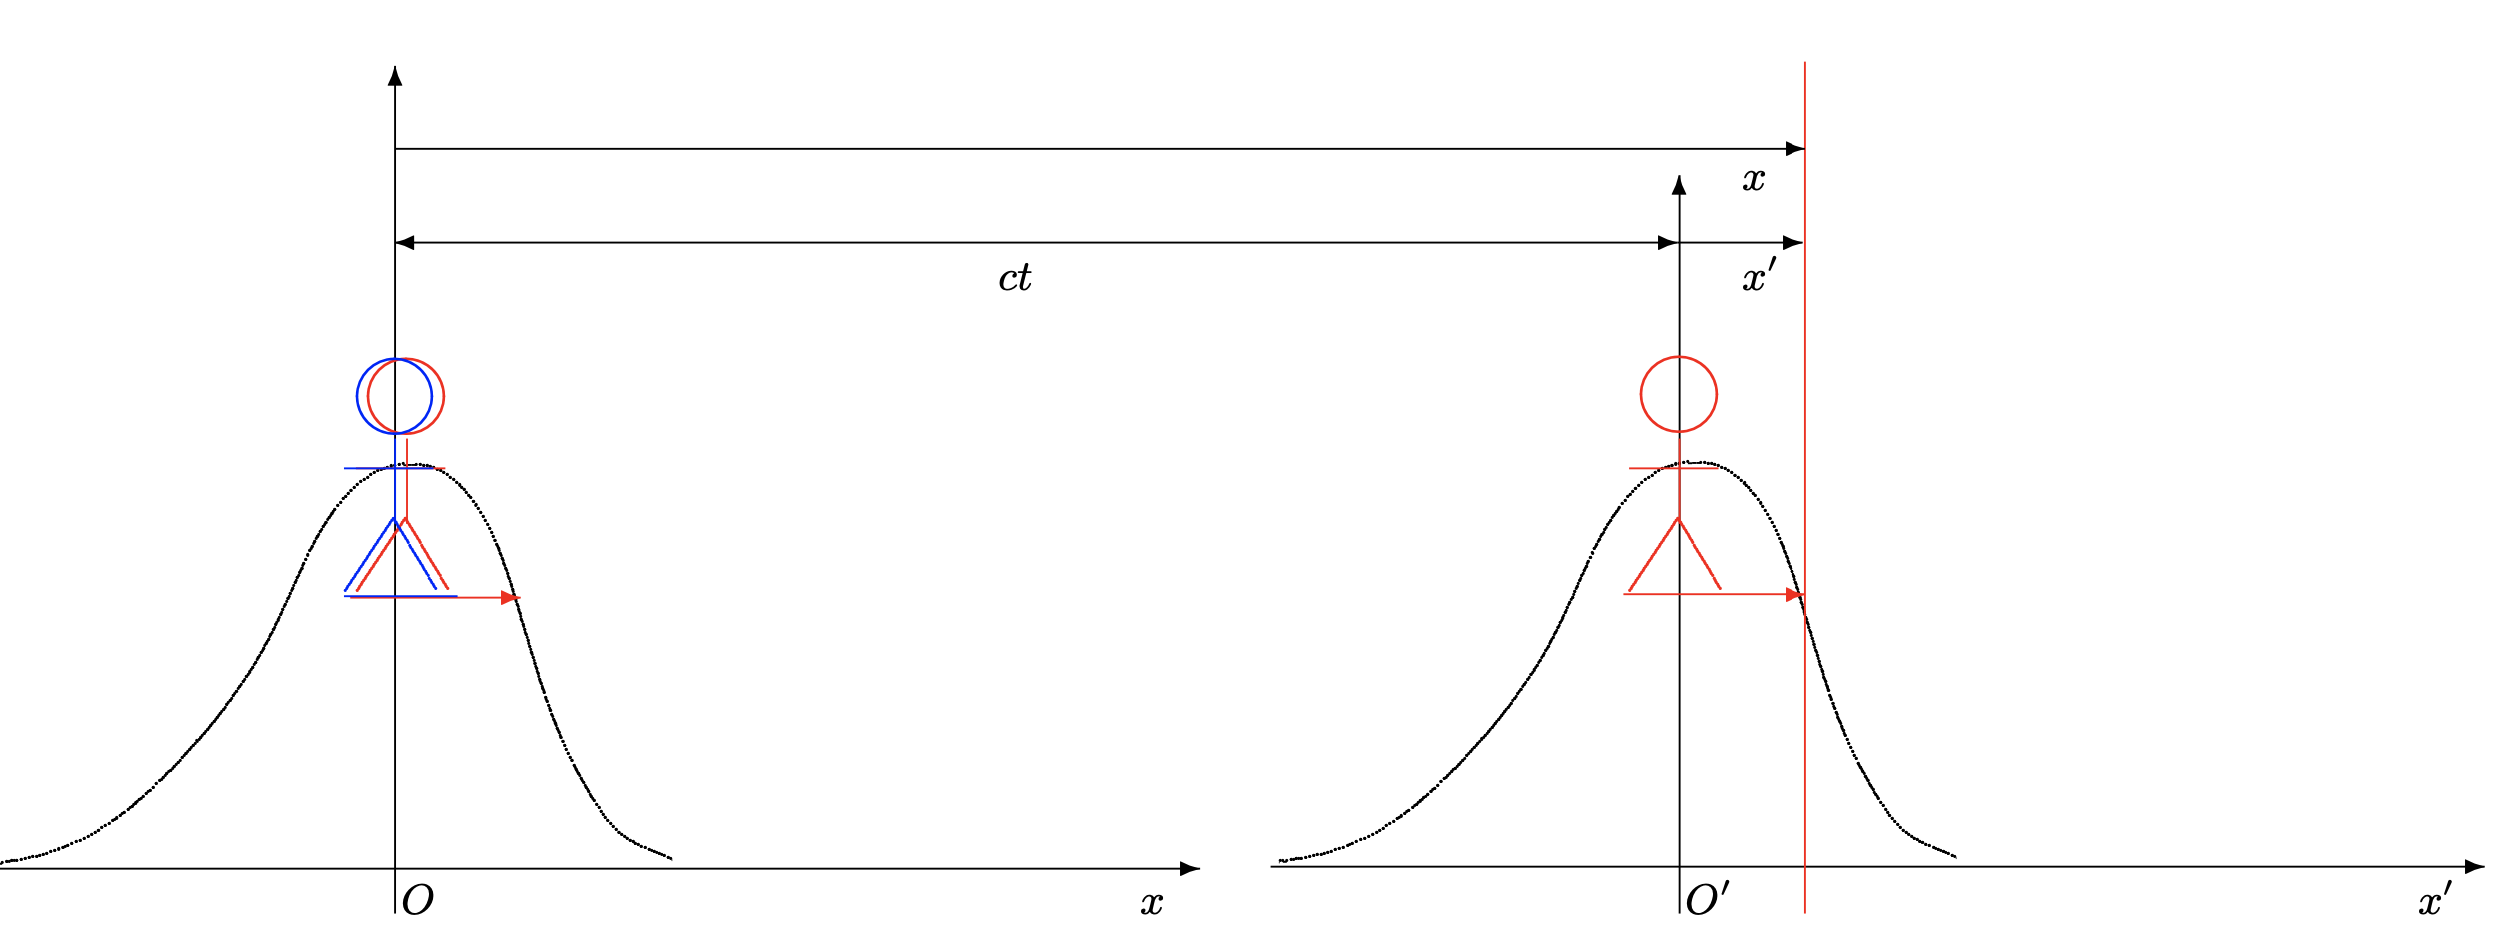
\includegraphics[scale = 0.3]{wave}
	            
	              \end{center}
	             可以理解为人随着wave移动,且将其位移分解为相对于底面和相对于wave:wave随时间移动$ct$,人相对于wave移动的距离是$x$,所以说对于$f(x - ct)$的意义实则是相对于地面得我总位移。而$u(x,t)$是描述了两者加总的影响。
	             
	             \smallskip
	             
	             For second case, it is called a \textit{convection-diffusion equation}. It depict a case that the wave not only moves to the right, it also diffuses along the way. 
	             
	            \bigskip
	            
	            \item \textbf{Second order wave function}
	            
	            \smallskip
	            
	            The expression in a operator form is
	            \[
	            (\frac{\partial}{\partial t} + c \frac{\partial }{\partial x})(\frac{\partial}{\partial t} - c\frac{\partial}{\partial x}) u(x,t) = 0
	            \]
	            this PDE depict a wave that is moving to both right and left side. Then opening the above equation we get 
	            \[
	            \frac{\partial^2 u}{\partial t^2} - c^2 \frac{\partial^2 u}{\partial x^2} = 0
	            \]
	            
	            \textcolor{blue}{more?}
	            
	            \medskip
	            
	            \item \textbf{Heat/Diffusion Equation}
	            
	            \smallskip
	            
	            Consider the heat conduction in a length $\Delta x$ conducting bar. Some notations we use here is $u(x,t)$ is the temperature at location $x$ , time $t$; $q(x,t)$ is the heat energy flux, defined to be heat energy per unit area; $C$ is the constant indicting the heat capacity, defined as the \textit{amount of energy needed to increase the temperature of 1 kilogram of the material by 1 kelvin degree}; $\rho$ is the density of the material and $A$ is the cross sectional area the bar.
	            
	                \medskip
	                
	                By the conservative law, which says \textit{the change must equal to the difference of flux in and out}, we know that the \textit{increase in thermal energy of the bar with length $\Delta x$  = the thermal energy in - thermal energy out}. Then the equation becomes 
	                \[
	                C[u(x, t + \Delta t) - u(x,t)] \cdot \rho \Delta x \cdot A = [q(x,t) - q(x + \Delta x, t)] \cdot A \Delta t
	                \]
	                divided by $A \Delta t \Delta x$ and let $\Delta \rightarrow 0$ 
	                \[
	                \rho C \cdot u_t + q_x = 0
	                \]
	                which is the conservative PDE for energy. Then we want to find a constitutive relation between $u$ and $q$. This can be achieved by using several physical theorems. 
	                \begin{enumerate}
	                
	                \medskip
	                
	                
	                \item  \textit{Fourier's Law}
	                
	                \smallskip
	                
	                This depict the truth that heat always flow from high temperature to low temperature.  The guessed solution is in form 
	                \[
	                q = k \cdot \frac{\partial u}{\partial x}
	                \]
	                where $k$ is the thermal conductive 导热性. This gives solution 
	                \[
	                u_t = \frac{k}{\rho C} u_{xx}
	                \]
	                common to call $k/\rho C$ the \textit{diffusion coefficient}.
	                
	                \smallskip
	                
	                \item \textit{Fick's Law}
	                
	                \smallskip
	                
	                The heat flows form the place of high concentration of energy to place of low concentration of energy. The valid guess here should be 
	                \[
	                q = -\alpha^2 (\rho C \cdot u)_x
	                \]
	                 where $\alpha$ is the diffusion coefficient. Plug into the PDE, the solution become 
	                 \[
	                 u_t = \alpha^2 u_{xx}
	                 \]
	                 Actually the general form of heat equation is 
	                 \[
	                 \frac{\partial u}{\partial t} = \alpha(u_{xx} + u_{yy} + u_{zz})
	                 \]
	                 where $t$ is time and $(x,y,z)$ is the coordinate. \textcolor{blue}{Important application in fin. math BS model.} There is actually another way to generate the heat equation by random walk, in \textcolor{blue}{Lecture note 7, Peirces.}
	                 
	                 
	                 
	                 \medskip
	                 
  	                 \underline{\textbf{Solving for the hear equation}}
  	                 
  	                 \smallskip
  	                 
  	                 
  	                 \begin{enumerate}
  	                 	\item \textit{Method of Finite Difference}
  	                 	
  	                 	\smallskip
  	                 	
  	                 	This is by doing the forward difference in time (first order accuarcy) and central difference in space (2nd order accuracy). This will finally produce a scheme in terms of time and position. Then integrate the BC and IC into the equation and using Matlab we can find the approximation of the answer by setting the appropriate $\Delta t$ and $\Delta x$ (in this case is $\Delta t \leq \Delta x^2/ 2\alpha^2$, ensuring the stability of the solution).
  	                 	
  	                     \medskip
  	                     
  	                     \item \textit{Separation of Variables}
  	                     
  	                     \smallskip
  	                     
  	                     Let first assume the initial conditions to be the 
  	                     \[
  	                     BC: u(0,t) = 0, u(L,t) = 0
  	                     \]
  	                     \[
  	                     IC: u(x,0) = f(x)
  	                     \]
  	                     The method of S.V is simply assume the solution is in form of 
  	                     \[
  	                     u(x,t) = X(x) \cdot T(t)
  	                     \]
  	                     then 
  	                     \[
  	                      \frac{X''(x)}{X(x)} = \frac{\dot{T}(t)}{T(t)} = -\lambda^2
  	                     \]
  	                     The two ratios must equals to a constant, since one is a fun. of position and the other one is fun. of t, it is not possible for them having the same expression. Then sloving for $T(t)$ and $X(x)$, where 
  	                     \[
  	                     T(t) = e^{-\lambda^2\alpha^2 t} \cdot D
  	                     \]
  	                     and for $X(x)$ we use the method form 215, get 
  	                     \[
  	                     X(x) = A sin(\lambda x) + B cox(\lambda x)
  	                     \]
  	                     Then apply the BC, notice that we want a non-trvial solution. Then general solution is in form 
  	                     \[
  	                     u_n(x,t) = \sin(\frac{n\pi}{L} x) \cdot e^{-(\frac{n\pi}{L})^2\alpha^2 t} 
  	                     \]
  	                     Since the linear combinations are also solutions, so the most general solution is 
  	                     \[
  	                     u(x,t) = \sum^{\infty}_{n = 1} b_n\sin(\frac{n\pi}{L} x) \cdot e^{-(\frac{n\pi}{L})^2\alpha^2 t}
  	                     \]
  	                     What's more, the time initial condition should be considered here. It generates 
  	                     \[
  	                     f(x) = \sum^{\infty}_{n = 1}b_n \sin(\frac{n\pi}{L} x)
  	                     \]
  	                     here we need the \textit{Fourier Sine Series} to solving for the coefficient. 
  	                 \end{enumerate}
  	                 
	                 
	                 \bigskip
	                 
	                \end{enumerate}
	                
	                
	                \item \textbf{Wave equation}
	                 
	                  \smallskip
	                  
	                  Can be generated by the motion of a elastic bar. Let $u(x,t)$ be the displacement and  $\sigma (x,t)$ be the normal stress. The equation is in form of 
	                  \[
	                  \frac{\partial \sigma}{\partial x} = \rho \cdot u_{tt}
	                  \]
                     which is called the \textit{balance of linear momentem}. Then apply the conservative law to connect $u$ and $\sigma$. The relation is built by \textit{Hooke's Law}. What the law depict is the relationship between stress and strain (the relative displacement). Let $\mathcal{E}$ to be 
                     \[
                     \mathcal{E} = u_x
                     \]
	                 and the guessed valid solution to be 
	                 \[
	                 \sigma =  \mathcal{E} u_x 
	                 \]
	                 plug into the momentum balance we get 
	                 \[
	                 u_{tt} = C^2 \cdot u_{xx}
	                 \]
	                 where $C = \mathcal{E} /\rho$. This is a 2nd order 1D wave equation, which is exactly the same as what we generated at the very beginning in a manner of operator. \textcolor{red}{Details need to be made up} 
	                 
	                 \bigskip
	                 
	                 \item \textbf{Laplace Equation}
	            
	                 \smallskip
	                 
	                 考虑二维的情况:在一个磁场中有一个线圈,我们在二维坐标系中移动。可以得知nex flux必须等于零。所以可得PDE为
	                 \[
	                 u_x + v_y = 0
	                 \]
	                 where we define $u(x,y)$ and $v(x,y)$ as $x$ component and $y$ component of velocity. Then use \textit{Darcy's Law} to build the constitutive relation. The relation is stated as 
	                 \[
	                 u = - K \frac{\partial h}{\partial x}\,\,\,\,\,\,\, v = - K \frac{\partial h}{\partial y}
	                 \]
	                 where $K$ is the \textit{Hydraulic Conductivity} and $h$ is the \textit{Hydraulic head} unit is $m$ \textcolor{red}{质量?} The law states that the flow direction is from place with high hydraulic head to low hydraulic head. Substitute into the PDE we get the Laplace equation 
	                 \[
	                 h_{xx} + h_{yy} = 0
	                 \]
	              
	               \textcolor{red}{Make up}
	               
	               \medskip
	               
	               
	            
	            
	            
	            
	            
	            
	            
	            
	            \end{enumerate}
	               
	   	   	 	\end{enumerate}
	   	   	 	
	   	   	 	\cleardoublepage
	   	   	 	
	   	   	 	\textbf{Index}
	   	   	 	
	   	   	 	\begin{enumerate}
	   	   	 		\item \textbf{Inner product space \& Orthogonal functions}
	   	   	 		
	   	   	 		\smallskip
	   	   	 		
	   	   	 		Extend the concept of vector space to function. Consider a vector sapce consisting of functions. To construct this, we first define the so-called \textit{inner product space}
	   	   	 		\begin{definition}
	   	   	 			(Inner product space) \, The vector space $\mathcal{V}$ with a well-defined mechanism $<,>$ is called the inner product space, if the $<,>$ satisfies for and two vector $\bold{u}$, $\bold{v}$ $\in \,\mathcal{V}$
	   	   	 			\begin{itemize}
	   	   	 				\item \textit{Linearity}\,\,\,\,\,$<a \bold{u} + b \bold{v}, \bold{w}> = a<\bold{u},\bold{w}> + b<\bold{u},\bold{w}> $
	   	   	 				\item \textit{Symmetric}\,\,\,\,\, $<\bold{u},\bold{v}> = <\bold{v},\bold{u}>$
	   	   	 				\item \textit{Positive Definite}\,\,\,\,\, For any $\bold{u} \in \mathcal{V}$, $<\bold{u},\bold{u}> \geq 0$ and $<\bold{u},\bold{u}> = 0 \iff \bold{u} = 0$
	   	   	 			\end{itemize}
	   	   	 		\end{definition}
	   	   	 	\end{enumerate}



\end{changemargin}

\end{document}